\documentclass[12pt]{extarticle} 
\usepackage[T2A]{fontenc} 
\usepackage[utf8]{inputenc}
\usepackage[russian]{babel}
\usepackage{mathtext}
\usepackage{graphicx}
\usepackage{graphics}
\usepackage{caption}
\usepackage{subcaption}
\usepackage{amsmath}
\usepackage{amsthm}
\usepackage{lscape}
\usepackage{makecell}
\usepackage{multirow}
\usepackage{ulem}
\usepackage{indentfirst}
\usepackage{enumerate}
\usepackage{amssymb}
\usepackage{setspace}
\usepackage{titlesec}
\usepackage{epstopdf}
\usepackage{fancyhdr}
\usepackage{enumitem}
\usepackage[left=2.5cm, right=1cm, top=2cm, bottom=2cm]{geometry}

% redefine the plain pagestyle
\fancypagestyle{plain}{%
\fancyhf{} % clear all header and footer fields
\fancyhead[C]{\thepage} % except the center
}
\renewcommand{\headrulewidth}{0pt}

\titleformat{\section}{\normalfont\fontsize{14}{15}\bfseries}{\thesection}{1em}{}

\parindent=1.25cm
\pagestyle{plain}

%\usepackage{enumerate,letltxmacro}
%\LetLtxMacro\itemold\item
%\renewcommand{\item}{\itemindent1.25cm\itemold}

\begin{document}

\thispagestyle{empty}

\begin{center}

\textbf{МИНОБРНАУКИ РОССИИ\\
Федеральное государственное бюджетное образовательное \\
учреждение высшего образования\\
<<Ярославский государственный университет им. П.Г. Демидова>>\\}

\vspace{1cm}

\hspace{22em} На правах рукописи

\vspace{1cm}

\textbf{Научный доклад об основных результатах \\
подготовленной научно-квалификационной работы (диссертации) \\
на соискание ученой степени кандидата наук}

\vspace{0.5cm}

{\large
\textbf{<<Бифуркационные особенности одного класса \\
краевых задач параболического
типа со специальными краевыми условиями>>}
}

\vspace{1cm}

по направлению подготовки

\vspace{0.5cm}

09.06.01 Информатика и вычислительная техника

\vspace{1cm}

направленность (профиль)

\vspace{0.5cm}

05.13.18 --- Математическое моделирование, \\ 
численные методы и комплексы программ

\vspace{1cm}

\end{center}
	
\hspace{16em} Научный руководитель\par
\hspace{16em} д. ф.-м.н., профессор\par
\hspace{16em} \underline{\hspace{5cm}}С.Д. Глызин \par
\hspace{16em} "<\underline{\hspace{0.9cm}}">\underline{\hspace{4.9cm}}2019 г.\par
	
\vspace{0.5cm}
	
\hspace{16em} Аспирант\par
\hspace{16em} \underline{\hspace{4.3cm}}Л.И. Ивановский \par
\hspace{16em} "<\underline{\hspace{0.9cm}}">\underline{\hspace{4.9cm}}2019 г.\par
	
\vspace{1.5cm}
	
\begin{center}
	Ярославль 2019
\end{center}
	
\newpage

\begin{center}
{\Large \textbf{Общая характеристика работы}}
\end{center}

\hspace{0cm}

\hspace{0cm}

\hspace{0cm}

\section*{Актуальность темы исследования}

\hspace{0cm}

\hspace{0cm}

\hspace{0cm}

Эффективным инструментом познания разнообразных конкретных объектов и явлений окружающего нас мира служит теоретическое и численное исследование их математических моделей. Нередко для описания какого-либо физического или биологического процесса используются динамические системы, представленные системами дифференциальных уравнений. Примеры здесь могут быть обнаружены в сфере моделирования ассоциативной памяти, как например в книге Т. Кохонена [1], или в области популяционной динамики. 

Динамические системы являются объектом научных исследований вот уже несколько веков. Эта область математического моделирования развивается и до сих пор. Одним из ключевых вопросов в исследовании динамических систем является изучение устойчивости состояний равновесия. Решению данной задачи посвящена и значительная часть данной работы. Применение аналитических методов исследования наряду с численными позволило получить новые результаты для специальной нелинейной динамической системы с импульсными воздействиями и краевой задачи параболического типа со специальными краевыми условиями.

\hspace{0cm}

\hspace{0cm}

\hspace{0cm}

\section*{Степень разработанности темы исследования}

\hspace{0cm}

\hspace{0cm}

\hspace{0cm}

Перед проведением исследований велось изучение большого числа литературных источников. Среди научных трудов по теме исследования особое внимание уделялось серии статей за авторством Глызина С.Д., Колесова А.Ю., Розова Н.Х., посвященной релаксационным колебаниям и дискретным автоволнам в нейронных системах [2-6], а также книге Кащенко С.А. и Майорова В.В. о моделях волновой памяти [7]. Аналитические сведения, полученные из данных публикаций, послужили основой для численных исследований, речь о которых идет в первой главе диссертационной работы, посвященной нелинейной динамической системы с импульсными воздействиями. Помимо этого, на основе популяционных моделей из статьи Гурли С.А., Соу Дж.В.-Х., Ву Дж.Х. [8] и локальных методов анализа динамических систем из учебного пособия Глызина С.Д., Колесова А.Ю. [9] было проведено численное исследование краевой задачи параболического типа со специальными краевыми условиями. Ей посвящена вторая глава диссертационной работы. Для углубления знаний в области дифференциальных уравнений были также изучены научные труды Арнольда В.И. [10], Гукенхеймера Дж., Холмса Ф. [11], Катка А.\,Б., Хасселблата Б. [12] и Федорюка М.В. [13].

\section*{Цели и задачи исследования}

\hspace{0cm}

\hspace{0cm}

\hspace{0cm}

Объектами исследования диссертационной работы являются устойчивые режимы динамических систем. В рамках проведенных исследований изучалась устойчивость нулевого состояния равновесия краевой задачи параболического типа со специальными краевыми условиями, а также рассматривались перестройки, происходящие в фазовом пространстве нелинейной динамической системы с импульсными воздействиями.

Цель исследования заключается в изучении поведения устойчивых режимов с использованием аналитических и численных методов. Для достижения этой цели были сформулированы следующие задачи:

\begin{itemize}[leftmargin=1.5\parindent]

\item[--] Для специальной нелинейной динамической системы с импульсными воздействиями выделить области, соответствующие различным бифуркационным сценариям, и изучить перестройки, происходящие в фазовом пространстве соответствующего модельного отображения, в случае цепочки и кольца осцилляторов с диффузионным взаимодействием и кольца однонаправленно связанных осцилляторов. Для каждой области параметров проиллюстрировать полученные численные результаты.
\item[--] Для краевой задачи с краевыми условиями типа пространственного сдвига выявить критические зависимости параметров, при которых происходят дивергентная и колебательная потери устойчивости нулевого состояния равновесия. При значениях параметров, близким к критическим, построить нормальную форму и определить условия появления неоднородных состояний равновесия и циклов.

\end{itemize}

\hspace{0cm}

\hspace{0cm}

\hspace{0cm}

\section*{Научная новизна результатов}

\hspace{0cm}

\hspace{0cm}

\hspace{0cm}

По итогам проведенных исследований были получены следующие результаты:

\begin{enumerate}[label=\arabic*),leftmargin=1.5\parindent]
\item Для специальной нелинейной динамической системы с импульсными воздействиями, на координатной плоскости параметров были выделены области, соответствующие различным бифуркационным сценариям. Благодаря численному исследованию, в каждой из областей были изучены  перестройки, происходящие в фазовом пространстве соответствующего модельного отображения в случае цепочки, кольца и однонаправленной волны связанных осцилляторов.
\item Для краевой задачи с краевыми условиями типа пространственного сдвига были найдены критические значения параметров, при которых происходят различные бифуркации нулевого состояния равновесия. Полученные критические зависимости являются важнейшими элементами для построения областей значений параметров, определяющих устойчивость нулевого состояния равновесия краевой задачи. Также, при значениях параметров близких к критическим была построена нормальная форма и на ее основе были определены условия появления неоднородных состояний равновесия в одном случае и циклов в другом. 
\end{enumerate}

\hspace{0cm}

\hspace{0cm}

\hspace{0cm}

\section*{Теоретическая и практическая значимость проведенных исследований}

\hspace{0cm}

\hspace{0cm}

\hspace{0cm}

Полученные результаты исследований могут быть использованы специалистами в области нелинейной динамики, математической биологии и теоретической физики для решения широкого круга задач. Дополнительно найденные устойчивые режимы в ходе исследования нелинейной динамической системы с импульсными воздействиями могут быть использованы при моделировании ассоциативной памяти компьютера. Проведенный анализ устойчивости нулевого решения краевой задачи параболического типа со специальными краевыми условиями позволит модифицировать используемые в настоящий момент модели популяции живых существ, обитающих на прибрежных территориях.

\hspace{0cm}

\hspace{0cm}

\hspace{0cm}

\section*{Методология и методы исследования}

\hspace{0cm}

\hspace{0cm}

\hspace{0cm}

При выполнении исследований были использованы известные методы анализа бифуркаций и построения формул для режимов, ответвляющихся от неподвижных состояний равновесия. Однако искать неподвижные состояния сложных систем вручную, с использованием одного лишь аналитического аппарата практически невозможно, так как этот процесс сопряжен с большим количеством вычислений. Эффективным инструментом поиска устойчивых режимов в таком случае служит численное исследование. В связи с этим, были разработаны алгоритмы нахождения неподвижных состояний динамических систем, поиска дубликатов устойчивых режимов, вычисления амплитуды колебаний и построения фазовых портретов.

\newpage

\section*{Положения, выносимые на публичное представление}

\hspace{0cm}

\hspace{0cm}

\hspace{0cm}

\begin{enumerate}[label=\arabic*),leftmargin=1.5\parindent]
\item Выделенные области, соответствующие разным бифуркационным сценариям в случае цепочки, кольца и однонаправленной волны связанных осцилляторов.
\item Установленные множества значений начальных параметров, при которых возможно единовременное сосуществование большего числа устойчивых неподвижных точек для динамическим систем с импульсными воздействиями.
\item Перестройки, происходящие в фазовом пространстве модельного отображения в случае цепочки и кольца осцилляторов с диффузионным взаимодействием и кольца однонаправленно связанных осцилляторов.
\item Критические зависимости параметров, при которых происходят различные бифуркации нулевого состояния равновесия краевой задачи параболического типа со специальными краевыми условиями.
\item Уравнения амплитуды колебаний нулевого решения краевой задачи с краевыми условиями типа пространственного сдвига в случае дивергентной и колебательной потери устойчивости.
\end{enumerate}

\hspace{0cm}

\hspace{0cm}

\hspace{0cm}

\section*{Апробация результатов исследования}

\hspace{0cm}

\hspace{0cm}

\hspace{0cm}

По теме работы было опубликовано 6 статей, в том числе и две, входящие в перечень журналов ВАК, а также 15 тезисов докладов. 

Результаты исследований были представлены на следующих конференциях и конкурсах:
\begin{enumerate}[label=\arabic*),leftmargin=1.5\parindent]
\item Всероссийская конференция <<Методы суперкомпьютерного моделирования -- 2015>>, Таруса (9 -- 13.11.2015).
\item International Student Conference <<Science and Progress -- 2015>>, СПбГУ, Петергоф (17 -- 19.11.2015).
\item Внутривузовский конкурс проектов молодых ученых <<Молодежь и наука>>, ЯрГУ им. П.Г Демидова, Ярославль (18.02.2016).
\item XXIII Международная молодежная научная конференция студентов, аспирантов и молодых ученых <<Ломоносов -- 2016>>, МГУ им. М.В Ломоносова, Москва (11 -- 15.04.2016).
\item Всероссийский конкурс научно-технического творчества молодежи 

\vspace{-0.2cm}
<<НТТМ-2016>>, ВДНХ, Москва (12 -- 16.04.2016)
\item Всероссийская конференция <<Методы суперкомпьютерного моделирования -- 2016>>, Таруса (24 -- 26.05.2016).
\item XII Международная научная конференция <<БМК -- 2016>>, БГУ, Минск, Беларусь (5 -- 10.09.2016).
\item International Conference <<Supercomputer Simulations in Science and 

\vspace{-0.2cm}
Engineering>>, MIEM HSE, Moscow (6 -- 10.09.2016).
\item International Student Conference <<Science and Progress -- 2016>>, СПбГУ, Петергоф (17 -- 21.10.2016).
\item XXIV Международная молодежная научная конференция студентов, аспирантов и молодых ученых <<Ломоносов -- 2017>>, МГУ им. М.В Ломоносова, Москва (10 -- 14.04.2017).
\item VI International Conference <<The problems of mathematical physics and 

\vspace{-0.2cm}
mathematical modeling>>, NRNU MEPhI, Moscow (25 -- 27.05.2017).
\item Международная научная конференция <<Новые тенденции в нелинейной динамике>>, ЯрГУ им. П.Г Демидова, Ярославль (5 -- 7.10.2017).
\item International Conference <<Computer Simulation in Physics and beyond -- 2017>>, MIEM HSE, Moscow (9 -- 12.10.2017).
\item International Student Conference <<Science and Progress-2017>>, СПбГУ, Петергоф (13 -- 17.11.2017).
\item III Всероссийская (XVIII) молодежная научная конференция <<Молодежь и наука на Севере>>, ФМИ Коми НЦ УрО РАН, Сыктывкар (12 -- 16.03.2018).
\item XXV Международная молодежная научная конференция студентов, аспирантов и молодых ученых <<Ломоносов-2018>>, МГУ им. М.В Ломоносова, Москва (9 -- 13.04.2018).
\item International Conference <<Computer Simulation in Physics and beyond -- 2018>>, MIEM HSE, Moscow (24 -- 27.09.2018).
\item Международная молодежная научно-практическая конференция <<Путь в науку>>, ЯрГУ им. П.Г Демидова, Ярославль (2 -- 5.04.2019).
\item XXVI Международная молодежная научная конференция студентов, аспирантов и молодых ученых <<Ломоносов-2019>>, МГУ им. М.В Ломоносова, Москва (8 -- 12.04.2019).
\end{enumerate}

Помимо этого, было разработано приложение для изучения перестроек, происходящих в фазовом пространстве нелинейной динамической системы с импульсными воздействиями, а также программное обеспечение для расчета критических зависимостей параметров и амплитуды колебаний нулевого решения краевой задачи с краевыми условиями типа пространственного сдвига. Было получено 2 свидетельства о государственной регистрации программы для ЭВМ:

\begin{enumerate}[label=\arabic*),leftmargin=1.5\parindent]
\item Search relaxational cycles for maps, заявка \textnumero 2016615695 (дата регистрации: 26.07.2016).
\item Колебательное рождение пространственно-неоднородных режимов в краевой задаче с линейным отклонением, заявка \textnumero 2017619728 (дата регистрации: 28.11.2017).
\end{enumerate}

Часть работ была выполнена в рамках государственного задания Министерства образования и науки РФ, проект  \textnumero 1.1875.2014К и при поддержке гранта Российского научного фонда \textnumero 14-21-00158.

\hspace{0cm}

\hspace{0cm}

\hspace{0cm}

\begin{center}
{\Large \textbf{Основное содержание работы}}
\end{center}

\hspace{0cm}

\hspace{0cm}

\hspace{0cm}

\textbf{Во введении} определяются цели и основные задачи работы, обосновывается научная новизна, приводятся положения исследований, выносимые на защиту, а также указывается апробация полученных результатов.

\textbf{В первой части работы} изучалась система дифференциальных уравнений с запаздыванием, моделирующих слабое электрическое взаимодействие нейронов:
\begin{equation}\label{u_system} 
	\dot{u_j} = d(a_1u_{j-1}-a_2u_j+u_{j+1})+\lambda(-1+\alpha f(u_j(t-1)) - \beta g(u_j))u_j, \quad j = \overline{1,3},
\end{equation}
где $ a_1, a_2 \in \{ 0, 1, 2 \}, \, d , \beta \in \mathbb{R}_+, \, \lambda >> 1, \, \alpha > 1 + \beta $, а функции $ u_j=u_j(t) > 0 $ являются мембранными потенциалами нейронов. Эта система была основана на моделях из статей Глызина С.Д., Колесова А.Ю., Розова Н.Х. [2--4] и книги Кащенко С.А. и Майорова В.В. [7].  Параметры $ a_1, a_2 $, а также краевые значения потенциалов $ u_0 $ и $ u_4 $ могут быть связаны между собой следующими равенствами:

\begin{enumerate}[label=\arabic*),leftmargin=1.5\parindent]

\item $ a_1 = 1, \, a_2 = 2, \, u_0 = u_1, \, u_3 = u_4 $ в случае цепочки осцилляторов;
\item $ a_1 = 1, \, a_2 = 2, \, u_0 = u_3, \, u_1 = u_4 $ для кольца осцилляторов с диффузионным взаимодействием;
\item $ a_1 = 0, \, a_2 = 1, \, u_1 = u_4 $ в случае кольца однонаправленно связанных осцилляторов.

\end{enumerate}
Гладкие функции $ f(u), g(u) \in C^2(\mathbb{R}_+) $ удовлетворяют условиям:
$$ 0 < \beta g(u) < \alpha, \quad f(0) = g(0) = 1, \quad \forall u \in \mathbb{R}_+; $$
$$ f(u), g(u), uf'(u), ug'(u), u^2f''(u), u^2g''(u) = O(1/u) \quad \text{при} \quad u \to +\infty. $$
При сформулированных ограничениях система \eqref{u_system} допускает наличие синхронного цикла $ u_1 \equiv u_2 \equiv  u_3 = u_*(t, \lambda) $, где $ u_*(t, \lambda) $ --- устойчивое периодическое решение уравнения
\begin{equation}\label{sing_neuron}
	\dot{u} = \lambda(-1+\alpha f(u(t-1)) - \beta g(u))u,
\end{equation}
описывающего электрическую активность отдельного нейрона, периода
$$ T_*(\lambda): \quad \lim_{\lambda\to\infty} T_*(\lambda) = T_0, \quad T_0 = \alpha + 1 + (\beta+1)/(\alpha - \beta - 1). $$
Величина $ T_0 $ определяет главную часть периода устойчивого цикла одиночного осциллятора системы \eqref{u_system}. Существование и единственность требуемого цикла было доказано в работах Глызина С.Д., Колесова А.Ю., Розова Н.Х. [2, 3].

Для сингулярно возмущенной системы \eqref{u_system} в статьях Глызина С.Д., Колесова А.Ю., Розова Н.Х. [6, 7] с помощью замен

$$ u_1 = \mbox{exp}\left(\frac{x}{\varepsilon}\right), \quad u_j = \mbox{exp}\left(\frac{x}{\varepsilon} + \sum_{k=1}^{j-1}y_k\right), \quad j= 2,3, \quad \varepsilon = \frac{1}{\lambda}\ll 1, $$
где $ x, \, y_1, \, y_2 $ --- новые переменные, было доказано, что она сводится к системе обыкновенных дифференциальных уравнений без малых параметров, но с импульсными воздействиями:

\begin{equation}\label{y_system}
\begin{array}{l}
\dot{y_1} = d(e^{y_2} + a_1e^{-y_1} - e^{y_1} - a_1e^{-y_0}) \\
\dot{y_2} = d(e^{y_3} + a_1e^{-y_2} - e^{y_2} - a_1e^{-y_1})
\end{array}
\end{equation}
$$ y_j(+0) = \frac{\alpha -1}{\alpha - \beta - 1}y_j(-0), \quad y_j(1+0) = y_j(1-0) - \frac{\alpha}{\alpha - 1}y_j(+0), $$
$$ y_j(\alpha + 0) = (1 + \beta)y_j(\alpha - 0), \quad y_j(\alpha + 1 + 0) = y_j(\alpha + 1 - 0) - \frac{\alpha}{1 + \beta}y_j(\alpha + 0). $$
Значения переменных $ y_0, y_3 $ зависят от начальных условий на $ u_0 $ и $ u_4 $: 
\begin{enumerate}[label=\arabic*),leftmargin=1.5\parindent]
\item $ y_0 = y_3 = 0 $ в случае цепочки осцилляторов;
\item $ y_0 = y_3 = -(y_1 + y_2) $ для кольца осцилляторов с диффузионным взаимодействием;
\item $ y_3 = -(y_1 + y_2) $ в случае кольца однонаправленно связанных осцилляторов.
\end{enumerate}
Введем в рассмотрение отображение следующего вида
\begin{equation}\label{phi_z} 
	\Phi(z): \begin{pmatrix}
           z_1 \\
           z_2
          \end{pmatrix}
					\to
					\begin{pmatrix}
           y_1(T_0, z_1, z_2) \\
           y_2(T_0, z_1, z_2)
          \end{pmatrix},
\end{equation}
где $ y_1(-0, z_1, z_2) = z_1, \; y_2(-0, z_1, z_2) = z_2 $. Это отображение сопоставляет начальным условиям системы \eqref{y_system} решение с координатами $ y_1, \, y_2 $ в значении времени $ T_0 $. Для этого отображения справедлива

\newtheorem{theorem}{Теорема} 
\begin{theorem}
Любой грубой неподвижной точке $ z $ отображения \eqref{phi_z}, в системе \eqref{y_system} и как следствие в системе \eqref{u_system}, соответствует цикл периода $ T_0 $ с теми же свойствами устойчивости.
\end{theorem} 

\noindent Другими словами, согласно теореме 1, для того, чтобы говорить об асимптотически устойчивых циклах системы \eqref{y_system}, достаточно исследовать неподвижные точки отображения \eqref{phi_z}.

Асимптотический анализ отображения \eqref{phi_z} позволяет показать, что при достаточно малых значениях параметра $ d $ оно имеет как минимум четыре устойчивые неподвижные точки. При этом нулевое состояние равновесия устойчиво для любых значений $ d $. Ему соответствует однородный (синхронный) цикл системы \eqref{u_system}. Задача исследования состоит в определении таких значений параметров $ \alpha $ и $ \beta $, при которых отображение \eqref{phi_z} имеет наибольшее число устойчивых неподвижных точек. Также изучались вопросы перестроек, происходящих в фазовом пространстве отображения \eqref{phi_z}.

В результате численных исследований нелинейной динамической системы с импульсными воздействиями, на координатной плоскости параметров $ (\alpha, \beta) $ были выделены области $ A_1, \, A_2, \, A_3 $, соответствующие различным бифуркационным сценариям (см. рис. 1). 

\begin{figure}[h]
\begin{minipage}[h]{0.2\linewidth}
\center{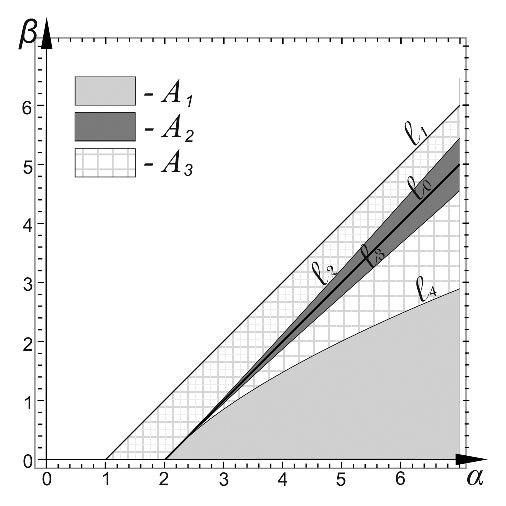
\includegraphics[scale=0.7]{chain.eps} \\ (a) }
\end{minipage}
\hspace{2.3cm}
\begin{minipage}[h]{0.2\linewidth}
\center{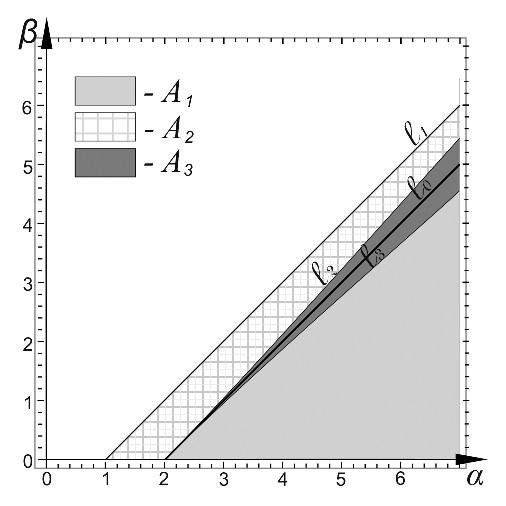
\includegraphics[scale=0.7]{ring.eps} \\ (b) }
\end{minipage}
\hspace{2.3cm}
\begin{minipage}[h]{0.2\linewidth}
\center{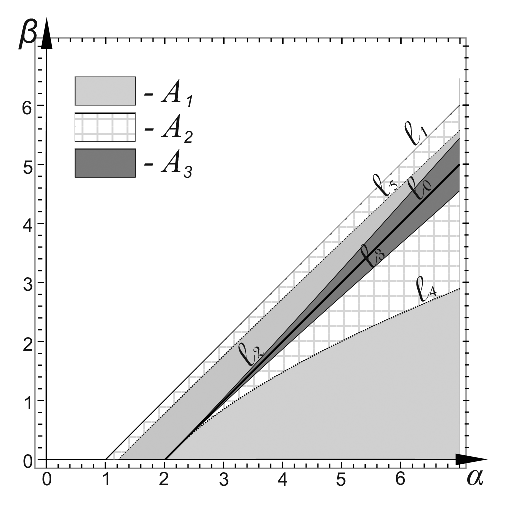
\includegraphics[scale=0.7]{wave.eps} \\ (c) }
\end{minipage}
\caption{ Области, соответствующие различным бифуркационным сценариям: (а) для цепочки осцилляторов, (б) для кольца осцилляторов с диффузионным взаимодействием, (в) для кольца однонаправленно связанных осцилляторов }
\end{figure}

Благодаря численному исследованию, в каждой из выделенных областей были подробно рассмотрены перестройки, происходящие в фазовом пространстве соответствующего модельного отображения. Особое внимание уделялось значениям начальных параметров, при которых возможно единовременное сосуществование большего числа устойчивых неподвижных точек. Для обнаружения различных состояний равновесия величины $ \alpha $ и $ \beta $ фиксировались, а значение $ d $ менялось.

\textbf{Во второй части работы} изучаются возникающие в проблематике популяционной динамики (см. работу Гурли С.А., Соу Дж.В.-Х., Ву Дж.Х. [8]) свойства краевой задачи параболического типа
\begin{equation}\label{boundary_problem}
	\dot u = u'' + \gamma u - \delta u^3,	
\end{equation}
cо специальным отклонением в одном из краевых условий
\begin{equation}\label{boundary_cond}	
	u'(0, t) \, = 0, \qquad u'(1, t) \, = F(u),
\end{equation}
где $ u(x, t) $ -- гладкая при $ t \geqslant 0 $ и $ x \in [0, 1] $ функция, а $ \gamma \in \mathbb{R} $. Отклонение $ F(u) $ и ограничение на параметр $ \delta $ выглядят следующим образом:

\begin{enumerate}[label=\arabic*),leftmargin=1.5\parindent]

\item $ F(u) = \alpha\,u(x_0, t), \, \delta>0 $, где $ \alpha \in \mathbb{R}, \, x_0 \in [0, 1) $ для нелинейной краевой задачи с линейным отклонением в краевом условии;
\item $ F(u) \, = \alpha\,u(x_0, t) + \beta u^3(x_0, t), \, \delta=0 $, где $ \beta \in \mathbb{R} $ для линейной краевой задачи с нелинейным отклонением в краевом условии;
\item $ F(u) \, = \alpha\int\limits_{0}^{1} u(t, y) dy, \,  \delta > 0$ для нелинейной краевой задачи с интегральным отклонением в краевом условии.

\end{enumerate}

Краевая задача \eqref{boundary_problem}, \eqref{boundary_cond} очевидным образом имеет нулевое решение. В зависимости от значений параметров, это решение может быть устойчивым или неустойчивым. Реализуется два способа потери устойчивости нулевого состояния равновесия --- дивергентный, когда в спектре устойчивости появляется нулевое значение, и колебательный, соответствующий случаю выхода пары собственных значений из левой комплексной полуплоскости на мнимую ось.

Задача исследования состояла в изучении свойств потери устойчивости нулевого решения краевой задачи \eqref{boundary_problem}, \eqref{boundary_cond}, т.е. в поиске критических значений параметров и построении асимптотических формул для режимов, от него ответвляющихся.

Для получения критических значений параметров изучалась линеаризованная в нуле краевая задача \eqref{boundary_problem}, \eqref{boundary_cond}. При выполнении замены вида $ u(x, t) = e^{\lambda t}v(x) $, можно получить краевую задачу на собственные значения $ \lambda $:
\begin{equation}\label{v_problem}
	v'' + (\gamma - \lambda)v = 0,	
\end{equation} 
Граничные условия для уравнения \eqref{v_problem} формируются путем подстановки стандартной эйлеровой замены в краевые условия \eqref{boundary_cond}.

Требуется определить, при каких критических значениях параметра $\alpha(\gamma)$  максимальная действительная часть собственных значений $ \lambda $ равна нулю. При подстановке $ \lambda = 0 $, в зависимости от вида функции $ F(u) $, в случае дивергентной потери устойчивости, можно получить аналитическую зависимость следующего вида:

\begin{equation}\label{a_u}
\alpha_u = \left\{
                \begin{array}{ll}
                  -\gamma, \; \mbox{при} \, F(u) \, = \alpha\int\limits_{0}^{1} u(t, y) dy, \\
                  \dfrac{ \sqrt{-\gamma} \, \sh \sqrt{-\gamma} }{ \ch \sqrt{-\gamma} x_0 }, \; \mbox{иначе}.
                \end{array}
              \right.
\end{equation}
В случае колебательной потери устойчивости, при $ \lambda = i \omega $, где $ \omega \in \mathbb{R} $, для критических значений $ \alpha $ получаем следующее выражение:
\begin{equation}\label{a_c}
	\alpha_c = \frac{ \sqrt{-\gamma + i \omega} \, \sh \sqrt{-\gamma + i \omega} }{ \ch \sqrt{-\gamma + i \omega} x_0 }.
\end{equation}
Отметим, что из-за особенностей краевых условий для нелинейной краевой задачи с интегральным отклонением реализуется только один, дивергентный способ потери устойчивости нулевого состояния равновесия.

Существует также иной способ получения зависимостей $ \alpha_u $ и $ \alpha_c $. Он связан с численным решением краевой задачи \eqref{boundary_problem}, \eqref{boundary_cond} и поиском таких критических значений $ \alpha $, при которых нулевое решение теряет устойчивость. Для этого рассматривается цепочка из $ n $ связанных осцилляторов, численно моделирующая краевую задачу \eqref{boundary_problem}, \eqref{boundary_cond}
\begin{equation}\label{numeric_problem} 
	\dot{u}_j =  n^2(u_{j+1} - 2u_j + u_{j-1}) + \gamma u_j, \quad j = \overline{1, n}, 
\end{equation}
где $ u_0 = u_1 $, а второе краевое условие заменяется на

\begin{enumerate}[label=\arabic*),leftmargin=1.5\parindent]

\item $ u_{n+1} = u_n + \frac{\alpha}{n}\:u_k $ для задачи с отклонением в краевом условии по координате $ x_0 $. Значение индекса $ k \in [1,n] $ соответствующего осциллятора $ u_k $ определяется, исходя из величины отклонения $ x_0 $;
\item $ u_{n+1} = u_n + \frac{\alpha}{n^2} \sum_{k=1}^{n} \:u_k $ для задачи с интегральным отклонением в краевом условии.

\end{enumerate}
При проведении численных экспериментов величина $ n $ считалась равной 50.

\newpage

Схематическая визуализация критических зависимостей \eqref{a_u} и \eqref{a_c} показана на рис. 2. Кривая $ \alpha_u $, соответствующая случаю дивергентной потери устойчивости нулевого состояния равновесия, изображена синим цветом, а кривая $ \alpha_c $, соответствующая случаю колебательной потери устойчивости нулевого решения краевой задачи \eqref{boundary_problem}, \eqref{boundary_cond}, показана красным цветом.

\begin{figure}[h]
\begin{minipage}[h]{0.2\linewidth}
\center{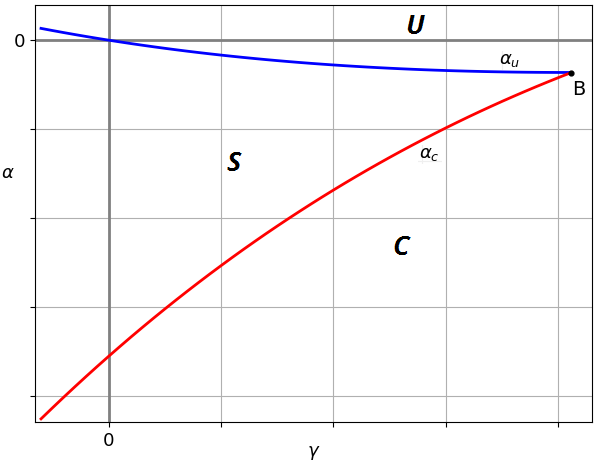
\includegraphics[scale=0.55]{scheme.png} \\ (a) }
\end{minipage}
\hspace{5cm}
\begin{minipage}[h]{0.2\linewidth}
\vspace{-0.2cm}
\center{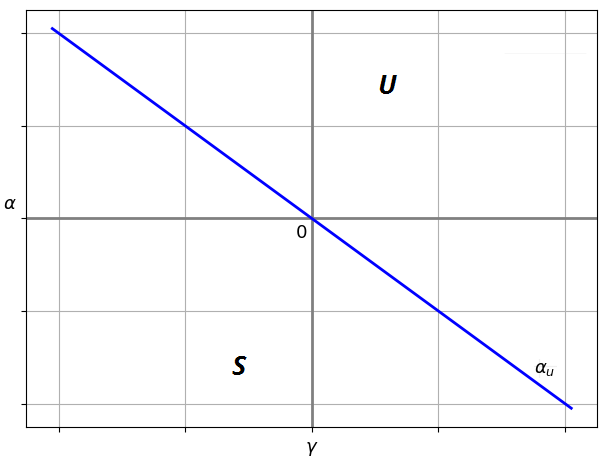
\includegraphics[scale=0.55]{alpha_u.png} \\ (b) }
\end{minipage}
\caption{ Схематическая визуализация кривых $ \alpha_u $ и $ \alpha_c $: (а) в случае отклонения в по координате $ x_0 $, (б) в случае интегрального отклонения }
\end{figure}

Кривые $ \alpha_u $ и $ \alpha_c $ являются важнейшими элементами для построения областей значений параметров $ \alpha $ и $ \gamma $, определяющих устойчивость нулевого решения краевой задачи \eqref{boundary_problem}, \eqref{boundary_cond}. Так область $ S $ соответствует случаю устойчивого нулевого состояния равновесия, $ U $ -- устойчивого, но отличного от нуля состояния равновесия, а в области параметров $ C $ наблюдается возникновение устойчивого многообразия вокруг нулевого решения.


Для изучения фазового портрета краевой задачи \eqref{boundary_problem}, \eqref{boundary_cond} в окрестности нулевого состояния равновесия, как и в учебном пособии Глызина С.Д., Колесова А.Ю. [9], используется нормальная форма, которая получается в результате разложения решения по степеням малого параметра $ \varepsilon $:
\begin{equation}\label{norm_form}
	u = \sqrt{\varepsilon}u_0 + \varepsilon u_1 + \varepsilon^{\frac{3}{2}} u_2 + O(\varepsilon^2).
\end{equation}
Параметр $ \varepsilon = | \alpha - \alpha_{cr} | $, где $ \alpha_{cr} $ -- критическое значение параметра $ \alpha $, косвенно характеризует собой отклонение от положения равновесия. Подстановка приведенного выше разложения в краевую задачу \eqref{boundary_problem}, \eqref{boundary_cond} приводит к системе последовательно разрешимых краевых задач

\begin{equation}\label{u_0}
u_0 = u_0'' + \gamma u_0
\end{equation}
\begin{equation}\label{u_2}
\dot u_2 + \frac{\partial u_0}{\partial s} = u_2'' + \gamma u_2 - \delta u_0^3,
\end{equation}
где функция $ u_0 $ в зависимости от способа потери устойчивости нулевого решения принимает вид
$$
    u_0 = \left\{
                \begin{array}{ll}
                  z(s) \ch \sqrt{-\gamma} x, \; \mbox{при} \, \lambda = 0,\\
                  z(s) e^{i \omega t} \ch \sqrt{-\gamma + i\omega}\, x + \overline{z(s)} e^{-i \omega t} \overline{\ch \sqrt{-\gamma + i\omega}\, x}, \; \mbox{при} \, \lambda = i\omega
                \end{array}
              \right.
$$
Граничные условия для уравнений \eqref{u_0}, \eqref{u_2} формируются путем подстановки формулы \eqref{norm_form} в краевые условия \eqref{boundary_cond}.
Решая краевые задачи \eqref{u_0}, \eqref{u_2} можно получить уравнение на амплитуду колебаний нулевого решения краевой задачи \eqref{boundary_problem}, \eqref{boundary_cond}, которое будет выглядеть следующим образом:
\begin{equation}\label{z}
z' = \phi z + d z |z|^2.
\end{equation}
Исходя из формул, полученных для коэффициентов $ \phi, \; d $, численно были построены зависимости $ \operatorname{Re}(\phi) $ и $ \operatorname{Re}(d) $ от параметра $ \gamma $, т.е. при значениях $ \alpha $, близких к критическим, на основе примененной нормальной формы, были определены условия появления неоднородных состояний равновесия в одном случае и циклов в другом.

\textbf{В заключении} работы формулируются выводы, обобщающие результаты исследования. 

\textbf{В приложении A} приводятся фрагменты кода приложения для изучения перестроек, происходящих в фазовом пространстве динамических систем с импульсными воздействиями.  

\textbf{В приложении B} содержатся фазовые портреты модельного отображения, построенные с помощью специально разработанного приложения.

\textbf{В приложении C} приводятся фрагменты программной реализации алгоритмов для расчета критических зависимостей параметров и амплитуды колебаний нулевого решения краевой задачи с краевыми условиями типа пространственного сдвига.

\textbf{В приложении D} содержатся графики критических зависимостей параметров и действительных частей коэффициентов уравнения на амплитуду колебаний.

\hspace{0cm}

\hspace{0cm}

\hspace{0cm}

\begin{center}
{\Large \textbf{Заключение}}
\end{center}

\hspace{0cm}

\hspace{0cm}

\hspace{0cm}

В результате проведенных исследований были выполнены все необходимые задачи исследования.

Для специальной нелинейной динамической системы с импульсными воздействиями, на координатной плоскости параметров были выделены области, соответствующие различным бифуркационным сценариям. Благодаря численному исследованию, в каждой из областей были подробно рассмотрены перестройки, происходящие в фазовом пространстве соответствующего модельного отображения в случае цепочки и кольца осцилляторов с диффузионным взаимодействием и кольца однонаправленно связанных осцилляторов. Также были установлены множества значений начальных параметров, при которых возможно единовременное сосуществование большего числа устойчивых неподвижных точек.

Для краевой задачи параболического типа со специальными краевыми условиями были найдены значения параметра $ \alpha $, при котором происходят различные бифуркации нулевого состояния равновесия. Полученные критические зависимости являются важнейшими элементами для построения областей значений параметров, определяющих устойчивость нулевого решения краевой задачи. При значениях параметра $ \alpha $, близких к критическим, был выполнен локальный анализ с помощью построения нормальной формы. На ее основе были определены условия появления неоднородных состояний равновесия в одном случае и циклов в другом.

\newpage

\begin{center}
{\Large \textbf{Список литературы}}
\end{center}

\hspace{0cm}

\hspace{0cm}

\hspace{0cm}

\begin{enumerate}[leftmargin=1.5\parindent]

\item Кохонен Т. Ассоциативные запоминающие устройства / Т. Кохонен. - М.: Мир, 1982.- 962 с.

\item Глызин С.Д., Колесов А.Ю., Розов Н.Х. Релаксационные автоколебания в нейронных системах. I / С.Д. Глызин, А.Ю. Колесов, Н.Х. Розов // Дифференциальные уравнения. - 2011. - Т. 47, \textnumero~7. - С. 919-932.

\item Глызин С.\,Д., Колесов А.\,Ю., Розов Н.\,Х. Релаксационные автоколебания в нейронных системах. II / С.Д. Глызин, А.Ю. Колесов, Н.Х. Розов  // Дифференциальные уравнения. - 2011. - Т. 47, \textnumero~12. - С. 1675-1692.

\item Глызин С.\,Д., Колесов А.\,Ю., Розов Н.\,Х. Релаксационные автоколебания в нейронных системах. III / С.Д. Глызин, А.Ю. Колесов, Н.Х. Розов  // Дифференциальные уравнения. - 2012. - Т. 48, \textnumero~2. - С. 155-170.

\item Глызин С.Д., Колесов А.Ю., Розов Н.Х. Дискретные автоволны в нейронных системах / С.Д. Глызин, А.Ю. Колесов, Н.Х. Розов  // Журнал вычислительной математики и математической физики. - 2012. - Т. 52, \textnumero~5. - С. 840-858. 

\item Глызин С.\,Д., Колесов А.\,Ю., Розов Н.\,Х. Моделирование эффекта взрыва в нейронных системах / С.Д. Глызин, А.Ю. Колесов, Н.Х. Розов  // Математические заметки. - 2013. - Т. 93, \textnumero~5. - С. 682-699.

\item Кащенко С.А., Майоров В.В. Модели волновой памяти / С.А. Кащенко, В.В. Майоров - М.: Либроком, 2009. - 288 с.

\item Гурли С.А., Соу Дж.В.-Х., Ву Дж.Х. Нелокальные уравнения реакции-диффузии с запаздыванием: биологические модели и нелинейная динамика / С.А. Гурли, Дж.В.-Х. Соу, Дж.Х. Ву // СМФН. - 2003. - Т. 1. - С. 84-120.

\item Глызин С.Д., Колесов А.Ю. Локальные методы анализа динамических систем: учебное пособие / С.Д. Глызин, А.Ю. Колесов. - Ярославль: ЯрГУ, 2006. - 92 с.

\item Арнольд В.И. Дополнительные главы теории обыкновенных дифференциальных уравнений / В.И. Арнольд. - М.: Наука, 1978. - 304 с. 

\item Гукенхеймер Дж., Холмс Ф. Нелинейные колебания, динамические системы и бифуркации векторных полей / Дж. Гукенхеймер, Ф. Холмс. - Москва-Ижевск: Институт компьютерных исследований, 2002. - 561 с.

\item Каток А.\,Б., Хасселблат Б. Введение в теорию динамических систем с обзором последних достижений / А.Б. Каток, Б. Хассельблат. - М.: МЦНМО, 2005. - 464 с.

\item Федорюк М.В. Обыкновенные дифференциальные уравнения / М.В. Федорюк. - М.: Наука, 1985. - 448 с.

\end{enumerate}

\newpage

\begin{center}
{\Large \textbf{Список работ, опубликованных аспирантом по теме НКР}}
\end{center}

\hspace{0cm}

\hspace{0cm}

\hspace{0cm}

\begin{enumerate}[label=\arabic*),leftmargin=1.5\parindent]

\item Ивановский Л.И., Самсонов С.О. Фазовые перестройки одной двумерной динамической системы с импульсным воздействием / Л.И. Ивановский, С.О. Самсонов // Модел. и анализ информ. систем. - 2014. - Т. 21, \textnumero~6. - С. 179-181.
\item Ivanovsky L.I. Stable regimes of dynamic systems with impulsive influences / L.I. Ivanovsky // 
Lobachevskii Journal of Mathematics. - 2017. - Vol. 38, No. 5. - P. 921-925.

\hspace{-1.25cm} Прочие работы:

\item Ивановский Л.И., Самсонов С.О. Динамика одного двумерного отображения и устойчивые режимы сингулярно возмущенной системы нейронного типа / Л.И. Ивановский, С.О. Самсонов // Вычисл. техн. в естеств. науках. Методы суперкомп. модел. - 2015. - \textnumero~2. - С. 121-132.
\item Ивановский Л.И. Динамические свойства одного класса импульсным систем / Л.И. Ивановский // Вычисл. техн. в естеств. науках. Методы суперкомп. модел. - 2015. - \textnumero~3. - С. 126-131.
\item Ивановский Л.И. Устойчивые режимы динамических систем с импульсными воздействиями / Л.И. Ивановский  // Динамические системы. - 2016. - Т. 6 (34), \textnumero~2. - С. 113-132.
\item Ивановский Л.И. Устойчивые режимы одного класса динамических систем с импульсными воздействиями / Л.И. Ивановский  // Вычисл. техн. в естеств. науках. Методы суперкомп. модел. - 2017. - \textnumero~4. - С. 35-42.

\end{enumerate}

\end{document}